\section{Censored arms and absolute spatial estimates}\label{R:cal:geometry-section}
The density-one uniform law will require a bound on the number of ways to
undo an insertion into a walk. Two proposed cuts are valid only if the
exterior arms remain disjoint when one is reflected back toward the other. We estimate this
constraint using independent irreducible histories stopped just before
they reach a prescribed height. Lemma~\ref{R:cal:survival} gives their
survival probability; the kernel calculation in
Section~\ref{R:cal:kernels} transfers it to weighted bridge families.
These are the inputs to the insertion argument in
Section~\ref{R:cal:refolding}.

We use the finite calibrated estimates of Section~\ref{R:cal:section},
with $a=3/4$, $\vartheta=1/4$, $d_*=4/3$, and $\alpha=9/16$.
The same histories also give an independent proof of the absolute
spatial estimates proved in Section~\ref{R:geo:section}. We include that
proof to retain a route from the calibrated inputs alone. Throughout,
$\mu(\omega)=\rho^{|\omega|}$ counts visited centers, ports carry no
weight, and the source is fixed. All masses precede normalization.

\subsection{Finite inputs and the rapid-travel bound}\label{R:cal:fast-section}

The absolute estimate supplied by this route is the following. It will
control upper tails and positive moments after the probability
normalizers have been identified.
\begin{theorem}[Absolute suppression of rapid travel]\label{R:cal:fast}
For every fixed sufficiently small $\xi>0$ there are $c,C>0$ such that the unnormalized critical mass of all plane self-avoiding walks rooted at a fixed center obeys
\begin{equation}
 \sum_{R\le {\rm diam}\,\omega\le 2R,\ |\omega|\le R^{d_*-\xi}}\mu(\omega)
       \ \le\ C\exp(-R^c).                                                   \label{R:cal:fast-mass}
\end{equation}
\end{theorem}
Here $|\omega|$ counts centers; changing to edge count changes the weight by a fixed factor. The proof will follow the survival and kernel estimates below. We first record the finite geometric inputs and their concentration consequences.
We will only need sufficiently large length/distance parameters; all constants below may change by fixed geometric/unit factors.

Keep horizontal integral levels $y$. We use \(B_m\asymp (1+m)^{-\vartheta}\), the exponential diameter cutoff for strict bridges in strips, \(\Pr(D>r)\le C r^{-a}\), \(1-\mathbb E\exp(-tH)\asymp t^a\) and \(1-\mathbb E\exp(-tL)=t^{\alpha+o(1)}\). In particular \(\Pr(H\ge r)\asymp (1+r)^{-a}\). For the lower tail comparison, in \(\mathbb E\min(1,H/T)\gtrsim T^{-a}\) the contribution of \(H<\delta T\) is at most \(C\delta^{1-a}T^{-a}\) by the upper bound integrated in height; take \(\delta\) sufficiently small.

\paragraph{Angular growth and finite chord moments.}
The finite calibrated input also supplies angular growth
\cite[Section~11, Recoverable half-plane growth]{compL}.
For two signed lattice normals making angle $\pi/3$, fix a sufficiently
small relative transverse tolerance $\gamma>0$. There are positive constants
$r_\gamma,K_\gamma,c_\gamma,C_\gamma,C_{1,\gamma}$ such that, for
$r\ge r_\gamma$ and each admissible grid target $S\ge K_\gamma r$,
the construction starts with prefixes at scale $r$ from the fixed source
port on the first wall and continues them to the exact wall of the second
normal at distance $S$, with terminal port free. All centers stay in the first open half-plane and strictly
before the target wall; the mass is at least
$c_\gamma S^{-1/4}(S/r)^{-C_{1,\gamma}}$ and the diameter at most $C_\gamma S$.
During continuation the transverse distance from the second-normal ray
through the selected prefix endpoint is at most $\gamma u$, where $u$
is the second-normal level measured from the original source.
The joining cuts are recovered as the first qualifying singly crossed
walls. The finite flux identity applies on the simple polygonal domains
used below; its coefficient at an exit is the real part of
$\exp(i(3/8)\,\mathrm{turn})$, after a fixed common phase rotation if needed.

Finally, the finite visit identity and planar nesting bound give
\cite[Proposition~11.1]{compL}
\begin{equation}
 \sum_{\substack{\omega\text{ a boundary chord in }Q_R}}
       \rho^{L(\omega)}L(\omega)\le C R^{25/12},
 \label{R:cal:box-moment}
\end{equation}
where $Q_R$ is a convex lattice domain with boundedly many sides and
diameter $O(R)$, and both boundary
ports are summed. Averaging over order-$R$ translates of a fixed boundary
source gives the $CR^{13/12}$ bound used below for paths of diameter at
most $R$. Using a growing diameter cutoff may add logarithmic factors; it
does not produce an unrestricted bounded-factor first bridge moment.

\paragraph{Concentration of independent increments.}
\begin{lemma}[Height and planar displacement atoms]\label{R:cal:atoms}
For $k\ge1$ independent whole irreducibles, with atoms taken on the actual
support lattice,

\[
 \sup_j\Pr(S_H(k)=j)\le C k^{-1/a},\qquad
 \sup_w\Pr(S_{(H,X)}(k)=w)\le C k^{-2/a}. 
\]
\end{lemma}
\begin{proof}
We first obtain a lower tail in the transverse direction. The angular
growth input constructs a positive family of strict bridges of height $h$
whose transverse endpoint displacement has magnitude at least $ch$.
Here are the two stages of that construction.

Start from the bottom port with normals $n=y$ and $u$ making angle
$\pi/3$, at scale $c_*h$. Continue to each exact $u$-level in
$[(2-2\delta_*)h,(2-\delta_*)h]$. Choose the fixed $\delta_*>0$ small,
then $c_*$ and the relative transverse error much smaller than
$\delta_*$. The initial part has diameter $O(c_*h)$, and the
$u$-normal ray gains $y$-height at slope $1/2$. Thus every path remains
in $0<y<h$ and ends at transverse distance at least $ch$, with remaining
height between $\delta_*h/4$ and $2\delta_*h$. Each target has mass
at least $c h^{-\vartheta}$.

Keep only the prefix to the first qualifying single-crossing $u$-cut
in that target bin, testing the confinement and terminal-position
conditions just stated. The total discarded suffix mass is at most
$\sum_{j\le Ch}B_j\le Ch^a$. Summing first over the order-$h$ targets
therefore leaves a family of distinct prefixes of mass at least a
positive constant. From each such prefix, use the angular construction
with normals $u,n$ to reach $y=h$ exactly. This extension lies strictly
beyond the selected $u$-cut, has diameter $O(\delta_*h)$, and has mass
at least $c h^{-\vartheta}$. Its starting scale is a small fixed
fraction of the remaining height, so its diameter constant is independent
of $\delta_*$. For small enough $\delta_*$, the full path remains in
$y>0$ and retains transverse displacement at least $c'h$. The joining
cut is recoverable. Hence
\[
 B_h\{|X_{\rm total}|\ge c'h\}\ge c h^{-\vartheta}.
\]

To pass from this bridge family to one irreducible, use
$|X_{\rm total}|\le\sum_i|X_i|$. On the displayed event,
$\sum_i\min(1,|X_i|/h)$ is bounded below by a positive constant.
The marked-reward identity and the bridge-mass bound give
\[
\begin{aligned}
 c h^{-\vartheta}
 &\le C\sum_{j\le h}\mathbb E_p[\min(1,|X|/h);H=j]
                \sum_{b+d=h-j}B_bB_d\\
 &\le C h^{2a-1}\mathbb E_p\min(1,|X|/h).
\end{aligned}
\]
Thus $\mathbb E_p\min(1,|X|/h)\ge ch^{-a}$.

The off-axis construction and the height estimate must now be combined
uniformly over directions. Put $f_r(z)=\min(1,|z|/r)$. For a unit vector
$(v_1,v_2)$ let $W=v_1H+v_2X$. Reflection in the starting normal preserves
the irreducible law and changes $X$ to $-X$. Since
\[
 f_r(A+B)+f_r(A-B)\ge f_r(A),\qquad
 f_r(A+B)+f_r(A-B)\ge f_r(B),
\]
and at least one $|v_i|$ is at least $1/\sqrt2$, we obtain uniformly in
$(v_1,v_2)$
\[
 \mathbb E f_r(W)\ge c r^{-a},\qquad p(|W|>r)\le C r^{-a}.
\]
For the second bound use $|W|\le C D$ with the fixed coordinate units.
Apply the first bound at scale $\delta r$. Choose fixed $\delta>0$ small
enough that $c\delta^{-a}>2C$. The contribution of $|W|>r$ is then absorbed.
The contribution of $|W|<c'r$ is at most
$C\delta^{-1}(c')^{1-a}r^{-a}$, by the integrated upper tail. Choosing $c'$
sufficiently small after $\delta$ proves
\[
 p(c'r\le |W|\le r)\ge c''r^{-a}
\]
with constants independent of the direction.

Let $\phi(t)=\mathbb E e^{it\cdot(H,X)}$. For small $t\ne0$ use the last
annulus in direction $t/|t|$ with $r=1/|t|$, and symmetrize against an
independent copy of bounded diameter. The absolute phase difference is
between $c'/2$ and $2$ for sufficiently small $|t|$. Consequently
\[
 1-|\phi(t)|^2=\mathbb E[1-\cos(t\cdot((H,X)-(H',X')))]
       \ge c|t|^a.
\]
The random vector $(H,2X)$ lies in $\mathbb Z^2$. Its support differences
have rank two: otherwise a nonzero projection would be constant, contrary
to the directional annuli. A rank-two subgroup of $\mathbb Z^2$ has finite
index. Hence on the Fourier torus $|\phi|=1$ at finitely many points.
At each such point all support phases agree, so the modulus nearby is a
translate of the modulus at zero; on the compact complement it is uniformly
less than one. Fourier inversion thus bounds every atom by a constant times
\[
 \int_{\mathbb R^2}e^{-ck|t|^a}\,dt=C'k^{-2/a}.
\]
The one-dimensional argument for $H$, allowing its own finite set of peaks,
gives $Ck^{-1/a}$. No conditioning on the length of any irreducible has
been used.

\end{proof}

\begin{lemma}[Short bridges at a specified height]\label{R:cal:short}
For fixed small \(\delta>0\), some \(v_0,\sigma_0>0\) give uniformly for \(S^{1-v_0}/2\le m\le C S\),
\begin{equation}
 B_m\big(|\omega|\le S^{d_*-\delta}\big)\le C m^{-\vartheta} S^{-\sigma_0}.          \label{R:cal:short-height}
\end{equation}
\end{lemma}
\begin{proof}
Here and below $B_m(\cdot)$ denotes restricted bridge mass.
First sum over counts $k>m^{a-\theta}$. Exponential damping in length
bounds the short-length event by
\[
 p\{S_L(k)\le S^{d_*-\delta}\}
 \le \exp\{1-kq_L(S^{-d_*+\delta})\}.
\]
For $m\ge S^{1-v_0}/2$, choose $\theta,v_0>0$ sufficiently small
after $\delta$. The exponent is then at most $-S^c$ for some $c>0$.
There are at most $m$ counts.

For $k\le m^{a-\theta}$, put $t_0=m^{1-z}$ with $0<z\ll\theta$.
If all height jumps are at most $t_0$, positive exponential weighting
bounds the probability of attaining $m$ by
\[
 e^{-m/t_0}(1+C t_0^{-a})^k
 \le \exp\{-m^z+C m^{-\theta+az}\},
\]
which is smaller than every inverse power of $m$. Otherwise select a
jump exceeding $t_0$ and apply the height atom bound to the other
increments. Its cost is at most
$Ck m^{-a(1-z)}k^{-1/a}$; for $k=1$, the height tail gives the same
bound directly. Summing these terms yields
\[
 C m^{-a(1-z)}\sum_{k\le m^{a-\theta}}k^{1-1/a}
 \le C m^{a-1-\theta(2-1/a)+az}.
\]
Since $2-1/a>0$, choose $z$ so that the exponent has a fixed saving
below $a-1=-\vartheta$. The comparison $m\ge S^{1-v_0}/2$ turns
that saving into $S^{-\sigma_0}$, as required.

\end{proof}

\subsection{Two censored arms}\label{R:cal:censored}

\begin{lemma}[Censored two-arm survival]\label{R:cal:survival}
Start two independent sequences of irreducibles from the same bottom port \(p\) with first center \(v\). On each keep its history of completed pieces up to heights \textbf{strictly less} than \(g\), not including the first jump reaching or passing \(g\). Fix roles left, right. Impose the following constraints whenever \(0<d_1<d_2<g\) are cut heights in the left, right history respectively. The prefixes to them, apart from the shared start through \(v\), must go disjointly (leaving \(v\) on the two respective sides). At level \(d_1\) all crossings of the right prefix must be to the right of \(x_1\), the terminal horizontal coordinate of the left prefix. Write \(f(g)\) for the probability of these constraints. Then for each \(\eta>0\)
\begin{equation}
 f(g)\le C_\eta (1+g)^{-a+\eta}.                                             \label{R:cal:survival-bound}
\end{equation}

\end{lemma}

\begin{figure}[ht]
\centering
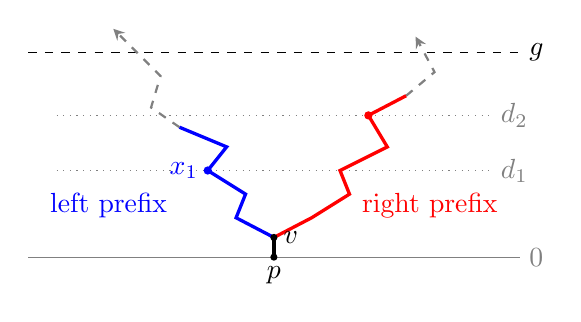
\begin{tikzpicture}[x=1.2cm,y=1cm,>=stealth]
 \draw[gray] (-2.6,0)--(2.6,0) node[right] {$0$};
 \draw[dashed] (-2.6,2.6)--(2.6,2.6) node[right] {$g$};
 \draw[gray,dotted] (-2.3,1.1)--(2.3,1.1) node[right] {$d_1$};
 \draw[gray,dotted] (-2.3,1.8)--(2.3,1.8) node[right] {$d_2$};
 \draw[very thick] (0,0)--(0,.25);
 \draw[very thick,blue] (0,.25)--(-.4,.5)--(-.3,.8)--(-.7,1.1)
    --(-.5,1.4)--(-1,1.65);
 \draw[very thick,red] (0,.25)--(.4,.5)--(.8,.8)--(.7,1.1)
    --(1.2,1.4)--(1,1.8)--(1.4,2.05);
 \draw[thick,gray,dashed,->] (-1,1.65)--(-1.3,1.9)--(-1.2,2.3)--(-1.7,2.9);
 \draw[thick,gray,dashed,->] (1.4,2.05)--(1.7,2.35)--(1.5,2.8);
 \fill (0,0) circle(1.3pt) node[below] {$p$};
 \fill (0,.25) circle(1.3pt) node[right] {$v$};
 \fill[blue] (-.7,1.1) circle(1.5pt) node[left] {$x_1$};
 \fill[red] (1,1.8) circle(1.5pt);
 \node[blue] at (-1.75,.65) {left prefix};
 \node[red] at (1.65,.65) {right prefix};
\end{tikzpicture}
\caption{The two histories share their first center $v$. Only complete
irreducibles ending strictly below $g$ are retained; the dashed continuations
are the omitted crossing pieces. At a tested left renewal level $d_1$, all
crossings of the right prefix ending at a higher tested level $d_2$ must lie
right of $x_1$. The paths are schematic, rather than lattice embeddings.}
\label{R:cal:censor-figure}
\end{figure}

\begin{proof}
There are two estimates to combine. A test with substantial transverse
clearance is rare by a positive flux comparison. After any candidate for
the last such test, each later test costs a power through either a large
height increment or a small transverse interval. Those later costs use
fresh coordinate blocks.

\paragraph{Test scales.}
Put $s=g$ large. Fix constants $0<\ell\ll\lambda\ll b\ll\kappa_0\ll1$, in particular
$b>2\lambda$, $\lambda\ge\ell$, and
$\kappa_0>b+2\lambda+a\ell$. These inequalities ensure that the normal
heights are separated, all tests lie below $g$, and each proximity test has
the saving used below. Use \(r_j=s^{\kappa_0+j\ell}\), \(0\le j\le J=\lfloor(1-2\kappa_0)/\ell\rfloor\). Test at piece indices sampled independently, uniform over integers \([A_{i,j}^a,2A_{i,j}^a]\) on the two uncensored sequences, where \(A_{1,j}=r_j,\ A_{2,j}=r_j s^b\) respectively. These index ranges are increasing and separated for large \(s\). Write \(d_i\) at a test for its cumulative heights; call them normal if each is in \([A_{i,j}s^{-\lambda}, A_{i,j}s^\lambda]\), implying \(1\ll d_1\ll d_2<g\). The chance of falling below such a range at any test is superpolynomially small by height damping. At normal heights we may also require both prefix diameters at most \(d_i\log^2 s\), except at superpolynomially small cost (sum the exponential strip diameter tail at the possible exact heights; a prefix at the given index has precisely its irreducible-product mass).

\paragraph{Separated tests and positive flux.}
Call a test separated if these normality, diameter and two-prefix constraints hold and the horizontal clearance between \(x_1\) and the leftmost right-prefix crossing at \(d_1\) is at least \(\chi d_2\), where \(\chi=s^{-\kappa_0}\). Unconditionally, its probability is at most
\begin{equation}
 C r_j^{-a}s^{\kappa_0+a\lambda}(1+\log s)^C.                               \label{R:cal:separated-test}
\end{equation}
Here are the gluing details. Sort \(d_2\) into dyadic bins \(d_2\asymp H\). Translate both paths together so the line at \(d_1\) becomes \(y=0\), and a lattice corner chosen strictly in the clearance gap becomes the origin; this allows at least \(c\chi H\) placements per input. The top line is now \(y=\Delta=d_2-d_1\asymp H\). Work inside a parallelogram of triangles with this top, bottom at \(-C H\) (rounded outward), and slant side walls allowing all paths by width \(O(H\log^2 s)\) with ample margin. Slit it along \(y=0\) from its left wall to the origin (split the corresponding ports into two boundary copies). Joining the prefixes at \(v\), removing the common initial half-edge, gives a simple chordal arc from a top wall port to the lower lip of the slit. It has no other boundary contact. To mark the choice of \(v\) among deepest vertices, use the hexagonal face centered at the bottom-left corner of \(v\)'s triangle. Its only vertices at height \(\ge y(v)\) are \(v\), a second minimum-height candidate at its left, and their common higher neighbor. The edge from \(v\) to that neighbor is used; if the second candidate is visited it must also use its edge to the same neighbor (minimum height and not an endpoint). Thus exactly a contiguous one- or two-edge arc of the face is present. Replace by the complementary face arc, giving a unique deepest vertex and hence identifying the face. This lies far from the domain boundaries. The change and joining have bounded weight costs. Inverse multiplicity is bounded since we can undo at that face and recover both original prefixes by translating \(v\) back (and the slit placement is determined).

Figure~\ref{R:cal:slit-figure} shows the resulting domain and the clipping operation used in the flux comparison.

\begin{figure}[ht]
\centering
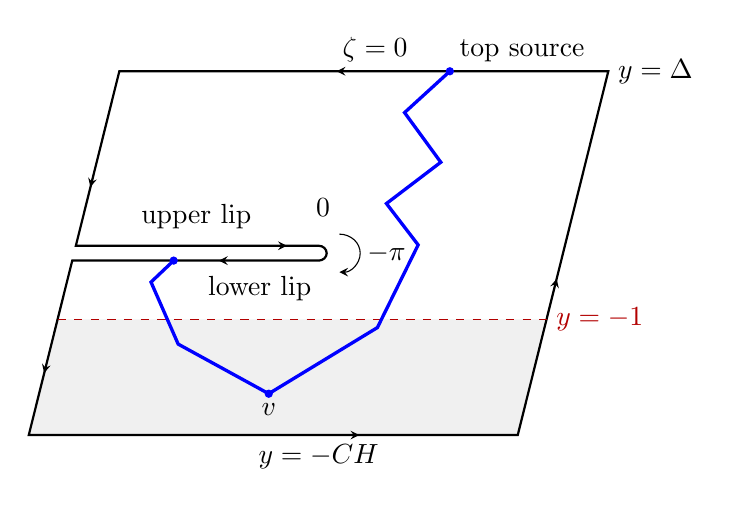
\begin{tikzpicture}[x=1.15cm,y=1.05cm,>=stealth]
 \fill[gray!12] (-2.882,-.8)--(2.518,-.8)--(2.2,-2.2)--(-3.2,-2.2)--cycle;
 \draw[thick] (1.45,2.2)--(-2.2,2.2)--(-2.68,.09)--(0,.09)
   arc[start angle=90,end angle=-90,radius=.09]
   --(-2.72,-.09)--(-3.2,-2.2)--(2.2,-2.2)--(3.2,2.2)--cycle;
 \draw[->] (1.05,2.2)--(.2,2.2) node[midway,above] {$\zeta=0$};
 \draw[->] (-2.35,1.54)--(-2.52,.8);
 \draw[->] (-1.1,.09)--(-.35,.09);
 \draw[->] (-.35,-.09)--(-1.1,-.09);
 \draw[->] (-2.84,-.61)--(-3.03,-1.45);
 \draw[->] (-.45,-2.2)--(.45,-2.2);
 \draw[->] (2.43,-1.18)--(2.63,-.31);
 \draw[->] (.23,.23) arc[start angle=90,end angle=-90,radius=.23];
 \node at (.75,0) {$-\pi$};
 \node[above] at (-1.35,.18) {upper lip};
 \node[below] at (-.65,-.16) {lower lip};
 \node[above] at (.05,.32) {$0$};
 \draw[red!70!black,dashed] (-2.882,-.8)--(2.518,-.8)
   node[right] {$y=-1$};
 \draw[very thick,blue] (1.45,2.2)--(.95,1.7)--(1.35,1.1)
   --(.75,.6)--(1.1,.1)--(.65,-.9)--(-.55,-1.7)
   --(-1.55,-1.1)--(-1.85,-.35)--(-1.6,-.09);
 \fill[blue] (1.45,2.2) circle(1.5pt) node[above right,black] {top source};
 \fill[blue] (-1.6,-.09) circle(1.5pt);
 \fill[blue] (-.55,-1.7) circle(1.5pt) node[below,black] {$v$};
 \node[right] at (3.2,2.2) {$y=\Delta$};
 \node[below] at (0,-2.2) {$y=-CH$};
\end{tikzpicture}
\caption{The slit domain for a separated test, before the bounded modification at the deepest face. The joined prefixes form the blue arc from the top source to the lower lip; their original common minimum $v$ lies below the clipping line. Boundary arrows specify the counterclockwise traversal, including its clockwise half-turn at the slit tip. The slit is drawn with positive thickness, and the vertical spacing is not to scale. The lifted-angle calculation in the proof supplies positivity of the flux coefficients.}
\label{R:cal:slit-figure}
\end{figure}

From each fixed top source, the mass in this slit domain of arcs as produced is \(\le C H^{-\vartheta}\). Indeed they are lost on clipping to \(y\ge-1\). The boundary extension identity from that source has uniformly positive real coefficients before and after clipping, unchanged to retained exit ports. Traversing counterclockwise starting west on the top, the lifted tangent travels down the left side, east along the upper lip, turns clockwise by \(\pi\) to west along the lower lip, continues down the left wall then around via the bottom, right wall and top. All lifted boundary tangent angles $\zeta$ relative to the start lie in
$[0,2\pi]$. Closing an arc along that boundary gives its turn as
$\zeta-\pi$: the two endpoint half-edge corners each add $\pi/2$.
Consequently its real flux coefficient is
$\cos((3/8)(\zeta-\pi))\ge\cos(3\pi/8)>0$, which supplies the required
uniform positivity.

More explicitly, the finite extension identity sums with the slit adjacencies forbidden (detour reversals valid since the source on the top is approached from outside any such cycle); slit ends of half-edges are boundary terms. For the simple arc turn calculation one can thicken the slit by an arbitrarily narrow indentation, trimming terminal half-edges at lip ports slightly if needed: other arc edges stay off the slit, including its corners, and the lifts at source and exit are as stated. Thus this also follows by closing in a simple boundary polygon.

Positive lost mass is bounded by the new exits' mass, and those exits are a subset of strict downward bridges of height \(\Delta+1\). This proves the claim. Summing over \(O(H\log^2 s)\) top ports and \(O(H)\) choices of \(\Delta\), and dividing by placements, gives \(O(\chi^{-1}H^a\log^2 s)\) cumulative input mass. The probability of each prefix pair at the test has, besides its bridge mass, index factors at most \(C r_j^{-a}(r_j s^b)^{-a}\) by uniform sampling (piece counts uniquely specified). Since \(H\le C r_j s^{b+\lambda}\), this gives \eqref{R:cal:separated-test}.

\paragraph{Fresh blocks after a candidate last separated test.}
Choose an index $p_0$ and require only that its test is separated.
Condition on all sampled indices and on both sequences through the test
at $p_0$. We do not condition on its being the last separated test.
For $p_0=-1$, expose no increments. We bound the event that the
survival constraints hold and that no later test is separated.

At every $j>p_0$, either a cumulative height exceeds
$A_{i,j}s^\lambda$, or the test has normal heights and its left endpoint
lies within $\chi d_2$ to the left of the minimum right-prefix crossing
at level $d_1$. The small-height and excessive-diameter cases were
already discarded. In the large-height case, some fresh index block
$q$, with $p_0<q\le j$, has gained at least $c_J A_{i,j}s^\lambda$.
The exposed height at $p_0$ is negligible compared with this threshold.
Assign such a side and block to the test; there are only a bounded
number of assignments, since $J$ is fixed. If several tests select one
block, keep its requirement for the largest $j$.

A block on side $i$ has at most $2A_{i,q}^a$ increments. The height-sum
tail therefore bounds its assigned event by
\[
 C_J s^{-a((j-q)\ell+\lambda)}
 \le C_J s^{-a\ell(j-q+1)}.
\]
Thus this one block pays for every test in the index interval $[q,j]$.
For each index outside the union of these intervals we use the
transverse proximity condition instead.

To estimate a proximity test, fix the entire relevant right sequence
and all earlier left blocks. The last left block contains order
$r_j^a$ fresh increments, so its joint endpoint atom is at most
$Cr_j^{-2}$ by Lemma~\ref{R:cal:atoms}. There are at most
$Cr_js^\lambda$ allowed left heights. At each one, the right sequence
specifies a transverse interval of length at most
$s^{-\kappa_0}r_js^{b+\lambda}$, which is at least one and hence also
bounds the number of lattice sites up to a constant. This gives the
uniform conditional bound
\[
 C r_j^{-2}(r_js^\lambda)
                (s^{-\kappa_0}r_js^{b+\lambda})
 = C s^{b+2\lambda-\kappa_0}
 \le C s^{-a\ell}.
\]
The left blocks used here are distinct and have not been assigned
large-height events. Their bounds multiply after the right sequence
has been fixed. The required large-height estimates for the right
blocks then multiply by their independence. Integrating left blocks
in reverse order gives the same conclusion for assigned left blocks
and proximity tests together. If $\mathcal C$ is the union of assigned
index intervals, the resulting cost is at most
\[
 C_J s^{-a\ell|\mathcal C|}
       s^{-a\ell(J-p_0-|\mathcal C|)}
 = C_J s^{-a\ell(J-p_0)}.
\]
Overlaps between assigned intervals only improve this upper bound.

\paragraph{Combining the two estimates.}
Every surviving pair has either a last separated test or none. For a
candidate $p_0\ge0$, multiply its unconditional bound
\eqref{R:cal:separated-test} by the uniform fresh-block bound just
proved. For no separated test use that bound with $p_0=-1$. Summing
over the finitely many candidates gives
\[
\begin{aligned}
 f(s)
 &\le C_J s^{-a\ell(J+1)}
   +C_J\sum_{p_0=0}^J
       r_{p_0}^{-a}s^{\kappa_0+a\lambda}(1+\log s)^C
       s^{-a\ell(J-p_0)}
   +s^{-M}\\
 &\le s^{-a+O(\kappa_0)+o(1)}.
\end{aligned}
\]
Here $M$ can be arbitrarily large, accounting for the discarded cases.
Choose $\kappa_0$ and then the smaller parameters so that the exponent
loss is less than the prescribed $\eta$. Enlarging the constant covers
bounded $s$ and proves \eqref{R:cal:survival-bound}.

\end{proof}

\subsection{Summing the cores between censored ends}\label{R:cal:kernels}

The preceding lemma is a probability estimate for two independent
histories. A bridge of prescribed height does not have independent ends.
We now express its positive weight relative to the independent history
laws, keeping a kernel for the pieces between them. Uniform bounds on
that kernel will justify using the survival estimate in weighted counts.

\paragraph{Endpoint conventions and the retained turn constraints.}
Decompose a walk into weak bridges with center endpoints, allowing ties
in height and cuts at singly crossed wall ports. Extend each piece to
exterior wall ports with an outward half-edge and, if necessary, one
additional center at each end. At a turn the common vertex is a height
extremum, with both used edges pointing toward the interior. The same
outward port can therefore be used for both virtual extensions. At a
lower turn they both begin $p\to v$ and then leave on opposite slants,
as in Lemma~\ref{R:cal:survival}. Their virtual starts are allowed to
coincide. Multiplying the strict-piece weights costs at most $C^k$ for
$O(k)$ pieces, accounting for duplicated or added centers. Recording the
local extensions and trimming choices also costs $C^k$ and recovers
the original anchored walk. Each span changes by a bounded amount.

At a turn use either the vacuous threshold $g=1$ or a threshold well
below both adjacent heights. Then the tested prefixes and their
continuations stay before the far endpoint modifications. They are
disjoint after $v$ because they come from disjoint arms of the original
walk. For the order condition, continue the left prefix to its first
hit of the higher tested level $d_2$. This is a strip crosscut meeting
its renewal level $d_1$ only once. The right arm leaves $v$ to its
right and cannot cross it, so all right-prefix crossings at $d_1$ lie
to the right of the left endpoint. Thus the survival constraints hold.
Reflection or reversal handles other turns, with at most a constant
choice of roles per turn.

\paragraph{The density relative to independent histories.}
Write $T(t)=p(H\ge t)$ and $p_j=p(H=j)$. If $\xi$ is a list of
complete irreducibles of total height $b<g$, its probability as the
history censored before $g$ is
\[
 \mathsf P_g(\xi)=\mu(\xi)T(g-b).
\]
The extra factor records that the next, omitted jump reaches or passes
$g$. In particular $T(g-b)\ge c g^{-a}$.

Consider a strict bridge of height $h$. Let $\xi_L,\xi_R$ be the
histories read inward from its two ends, with heights $b<g_L$ and
$d<g_R$. Put $T_L=T(g_L-b)$ and $T_R=T(g_R-d)$. We choose the
thresholds so that $h-b-d\asymp h$. Relative to
$\mathsf P_{g_L}\otimes\mathsf P_{g_R}$, the remaining mass is bounded
by the sum of two kernels:
\[
\begin{aligned}
 K_h^{\rm same}(\xi_L,\xi_R)
   &=\frac{p_{h-b-d}}{T_LT_R},\\
 K_h^{\rm distinct}(\xi_L,\xi_R)
   &=\mathbb E\!\left[
        B_{h-b-d-Y_L-Y_R}\,;\ h-b-d-Y_L-Y_R\ge0
        \ \middle|\ Y_L\ge g_L-b,\ Y_R\ge g_R-d
      \right].
\end{aligned}
\]
Here $Y_L,Y_R$ are independent copies of $H$. In the first case the
same irreducible crosses both thresholds; in the second, the two
crossing irreducibles are distinct and the bridge between them has
height $h-b-d-Y_L-Y_R$. A total-length upper bound on the original
piece may also be imposed on this middle bridge, replacing $B_m$ by
its restricted mass. All other restrictions can be dropped for an
upper bound.

These formulas follow by irreducible factorization. They keep the
survival-tail denominators supplied by the censored laws; those factors
cannot be omitted when passing from probabilities to weighted bridges.
No final transverse coordinate is prescribed. The terminal port is
fixed by translating the reversed suffix to the end of the middle
piece, so there is no additional placement factor.

\paragraph{Integration rule for a chain.}
For a chain of pieces take the product reference measure $\mathsf P$
of all its left and right censored-history laws. Retain only the chosen
turn indicators $\mathbf1_{E_v}$. Each indicator involves a disjoint
pair of end histories, aligned at their common turn. Choose their
thresholds from coarse data, independently of the fine height variables
still to be summed. With $K_i=K_i^{\rm same}+K_i^{\rm distinct}$, the
weighted chain sum is bounded, up to its recorded $C^k$ endpoint cost,
by
\[
 \int \left[\sum_{\boldsymbol h\in\mathcal A}
                  \prod_i K_i(h_i;\xi_{i,L},\xi_{i,R})\right]
          \prod_v\mathbf1_{E_v}(\boldsymbol\xi)
          \,d\mathsf P(\boldsymbol\xi),
\]
where $\mathcal A$ denotes the retained height constraints. If the
bracket is at most $C_*$ uniformly in the histories, this is at most
\[
 C_*\prod_v f(g_v).
\]
Thus the order is: fix the histories, sum the kernels over fine heights,
and only then integrate the independent turn indicators. The physical
weighted bridge family itself is not asserted to have independent ends.
Both the volume bound below and the insertion-label argument use this
rule; the latter needs only its one-ended version.

\begin{proposition}[Critical mass in a bounded region]\label{R:cal:volume}
Let \(V_R\) denote the mass of all center walks from a fixed center with diameter at most \(R\). We have for every \(\nu>0\)
\begin{equation}
 V_R\le \exp(C_\nu(1+R)^\nu).                                                \label{R:cal:volume-bound}
\end{equation}
\end{proposition}
\begin{proof}
Split at a lowest point (polynomial placement cost), then decompose each direction into weak bridges by repeatedly cutting at the last occurrence of the opposite extremum of the remaining path. On each chain spans are decreasing, strictly except possibly the second equal to the first. Group consecutive spans in dyads \([s,2s)\). In such a group of size \(k\), \(1\le k\le C s\), only impose shared-turn constraints \emph{within} the group. Strict heights \(h\asymp s\) there differ only boundedly from the weak spans. Assume \(s\) large (bounded small dyads cost a constant by the ordinary bridge bounds); take common threshold \(g=\max(1,\lfloor c_*s/k\rfloor)\asymp s/k\) for small fixed \(c_*\).

Call a piece exceptional in this sum if the threshold jumps coincide or are distinct with middle height \(m<g\). Its kernel summed over the height dyad costs at most \(C s^a k^{-2a}\). Indeed the coincident case uses the tail at \(h-b-d\gtrsim s\) summed at distinct heights, and the two \(T\) factors. In the other case one jump is of order \(s\), giving conditional probability \(\le C(g/s)^a\); sum also \(\sum_{m<g}B_m\le Cg^a\). For ordinary pieces (\(m\ge g\)) the kernel per fixed \(h\) costs \(\le C s^{-\vartheta}\): for \(m\asymp s\) this is direct, for \(m\) smaller use \(B_m\le C g^{-\vartheta}\) and the large jump factor \((g/s)^a\) again. For \(t=k-r\) ordinary pieces with \(r\) exceptional, we retain height ordering constraints among just the ordinary ones, giving at most \(C^k s^t/t!\) ordinary lists (original spans are ordered on the discrete grid, \(t\le Cs\), and bounded perturbations cost boundedly per piece). Exceptional heights sum without ordering. Multiply now by \(k-1\) pair factors \eqref{R:cal:survival-bound}. Uniformly from the fixed group start the total, absorbing subset choices, is at most
\[
 C_\eta^k s^{ak}\, k^{-2ar}(t!)^{-1}\,(s/k)^{(-a+\eta)(k-1)}
       \le s^a\big(C'_\eta s^\eta/k^\vartheta\big)^k ,
\]
with the last bound also covering the sum over types (\(1/t!\le \exp(k)/k^t,\ 2a>1\)). Summing \(k\) and multiplying over \(O(1+\log R)\) dyads on each chain proves \eqref{R:cal:volume-bound}, taking \(\eta\) sufficiently small depending on \(\nu\) (terms with \(k\) above a constant times \(s^{2\eta/\vartheta}\) already decay). We overcount freely between groups/chains.

\end{proof}

\subsection{Subdivision for fast crossings}\label{R:cal:subdivision}

\begin{proof}[Proof of Theorem~\ref{R:cal:fast}]
An input of \eqref{R:cal:fast-mass} contains a weak bridge between a minimum and maximum in some signed normal direction of span \(H\asymp R\), since the three lattice directions control diameter; take the sign so it is oriented from low to high. We call this coordinate \(y\) again. The exterior pieces cost at most \(V_{2R}^2\) up to constants; it suffices to estimate such weak bridges from their fixed first vertex. Pay \(O(R)\) for specifying the last height and normalize the first height by translation.

Take \(\delta=\xi/2\), small \(0<\sigma\ll\xi\), integer \(S\asymp R^{1-\sigma}\), so \(R^{d_*-\xi}=o(S^{d_*-\delta})\). First divide the bridge into swings with drawdown/up threshold \(s_0=S/10\). Track running maxima from the beginning; on first detecting a fall by at least \(s_0\) from one, mark the last corresponding peak before detection and switch to tracking running minima starting at detection, with next switch symmetrically after a rise, marking the trough, and so on. Use the marked extrema (not the detection points) and the two endpoints to cut. Every resulting swing is a weak bridge of span \(\ge s_0\), with adverse increments between any earlier and later point of that swing strictly less than \(s_0\). Indeed, e.g. on an upswing the initial trough-to-rise-detection part lies above the trough, and strictly within \(s_0\) above it before detection. From detection to the peak the running maximum rule gives the bounds; all heights stay above the trough and at most the peak on both parts. The reversed argument works going down, and the global endpoint extrema handle first/last swings (after detecting a fall there must still be a rise by threshold before or at the terminal maximum). Without any switch the span itself is \(H\).

Inside each swing use all absolute grid levels spaced by \(S\) (multiples of \(S\) in wall coordinates) with interior margin \(\ge 2s_0\) from both extrema. Here is the subdivision in upward orientation, symmetrically otherwise. For each such level \(l\), if there is just one crossing, cut there at the port. Otherwise take a highest vertex \(A_l\) before the last upward crossing of \(l\), and a lowest \(B_l\) after \(A_l\) in this swing. Then \(y(A_l)>l>y(B_l)\), both are between the first and last crossings (a return occurs after \(A_l\), all vertices after last crossing are above). The path between them is a descending weak bridge of span \(<s_0\); mark it as an inserted piece. These crossing zones for successive levels occur in order since a backtrack of size \(S\) is impossible. All intermediate pieces are upward weak bridges: e.g. from \(B_l\) to \(A_{l+S}\) all vertices respect those extremal bounds, with the analogous inequalities at single crossings and swing endpoints. These \textbf{main} pieces have spans between \(c S\) and \(C S\), by the margins, offsets \(<s_0\) and the minimum full swing span if no cut. Thus throughout the original bridge there are \(k\ge c H/S\) main pieces and at most \(k\) inserts.

Use strict virtual pieces with the bounded endpoint extensions described above. Specify their types/order, signs, and the following boundary data, at cost \(R^{O(1)}(C(1+\log R))^{C k}\) before any fine coordinates at turns:
\begin{itemize}
\item At a turn between swings, label the coarse height interval (grid of size \(S\)) and assign boundary scale \(D_j=S\).
\item At the two turns for an insert, label the grid level and a common dyad \(D_j\asymp 1+|y(A_l)-y(B_l)|\) (same at both). Each height has offset \(O(D_j)\) from that level.
\item At the single-cut ports label the grid level; take \(D_j=1\) there and at the prescribed endpoint heights.
\end{itemize}

Coarse coordinates cost boundedly many choices per piece from those before, since increments are \(O(S)\). We can include any finite endpoint/port adjustment types as labels. Thus each virtual boundary height \(w_j\) still to sum ranges over \(O(D_j)\) possibilities (already fixed at external endpoints and single cuts), and for fixed next \(w_{j+1}\) has bounded multiplicity per intervening strict-piece height \(h\), their signed difference. We restrict \(h\asymp P\), where \(P=S\) on main pieces, \(P=D_j=D_{j+1}\) on inserts; other fine height ordering restrictions will not be needed. Every strict piece length is \(\le S^{d_*-\delta}\) by the global input bound, including its bounded adjustments.

Use \eqref{R:cal:short-height}, and fix \(0<u\ll v\ll \min(v_0,\sigma_0)\). Call a boundary active if \(D_j\ge S^{1-v}\). At scale \(D'=D_j\) take the threshold
\[
 g(D')=\max(1,\lfloor c_*D'S^{-u\,{\bf1}_{\rm active}}\rfloor)
\]
for small fixed \(c_*\). Since each endpoint scale is \(O(P)\) this ensures \(h-b-d\asymp P\) at the censored kernel, and pair tests at turns are either vacuous or well below the adjacent far adjustments. Write \(F(D')=C_\eta g(D')^{-a+\eta}\) as a pair bound, or \(1\) at unpaired boundaries with \(D'=1\).

The subdivision has reduced rapid travel to many main pieces of scale $S$.
It remains to extract a power saving from each such piece without spending
the same independent end history twice.

We sum each kernel over its \emph{left} boundary height at fixed right height and histories from both ends (left/right here meaning first/last in traversal). Include in its numerical budget also the factor \(F(D_L)\) at the first boundary of that piece. We claim a bound \(S^{-c_1}\) for this product on main pieces and active-scale inserts, for some \(c_1>0\) uniformly at all sufficiently small \(\eta\); on inactive-scale inserts at most \(C_\eta S^{2\eta}\) suffices.

Indeed in the coincident-jump case the summed kernel is at most \(C g_L^a g_R^a P^{-a}\), using bounded multiplicity per height. With \(F(D_L)\) this leaves \(O_\eta(S^\eta (g_R/P)^a)\), giving the claim (on main pieces \(g_R/P\le C\max(S^{-v},S^{-u})\), and on active inserts \(\le CS^{-u}\)). In the distinct case sort \(1+m\) in dyads of scale \(M\). For fixed crossing increments each \(m\) can occur boundedly often as the left height varies, with \(O(D_L)\) possible heights total. Thus by \(B_m\le C M^{-\vartheta}\) we have kernel bound
\[
 C\min(D_L M^{-\vartheta},M^a)
   = C D_L^a\min((D_L/M)^\vartheta,(M/D_L)^a).
\]
Here \(D_L^a F(D_L)\le C_\eta S^\eta\) times \(S^{a u}\) if active. When \(M\ge S^{1-v_0}\) \eqref{R:cal:short-height} allows multiplying by \(S^{-\sigma_0}\), enough. For smaller \(M\) on a main piece or active insert, there must be a giant crossing jump \(y_i\ge cP\) on some side \(G\). Accordingly we can multiply the bound, after splitting into the two possible sides, by \(C (g_G/P)^a\) by its conditional tail. On a main piece this saves \(S^{-av}\) if \(G\) inactive, otherwise \(S^{-au}\); on an active insert (both sides active) also \(S^{-au}\). In the latter savings cases, if left itself is active and pays \(S^{au}\), the factor \((M/D_L)^a\le S^{-a(v_0-v)}\) supplies the gain. Inactive inserts just use the unconstrained dyad estimate with both boundary scales inactive. For clarity, all these cases have a common strictly positive saving before
the small $\eta$ loss:
\[
 \Lambda=\min\{au,\ a(v-u),\ a(v_0-v),\ \sigma_0-au\}>0.
\]
Every dyad on a main piece or active insert costs at most
$C_\eta S^{\eta-\Lambda}$. Choose $\eta$ sufficiently small, then sum
$O(\log S)$ dyads. This proves the claimed negative power; inactive inserts
cost at most $C_\eta S^{2\eta}$.

To combine, first hold all histories fixed and sum out the fine variables in sequence from first to last using the uniform summed-kernel bounds (the last height fixed). Applying the pair constraints \eqref{R:cal:survival-bound} in the product of censored-history probabilities contributes exactly the indicated upper costs allocated to the left boundaries. Taking \(\eta\) small, all labeling costs, inactive inserts, and endpoint weight factors are absorbed: the resulting weak-bridge sum is at most \(R^{O(1)}\sum_{k\ge cH/S} S^{-c_2 k}\) for some \(c_2>0\). This is stretched-exponentially small; \eqref{R:cal:volume-bound} at the two exterior pieces preserves this, proving \eqref{R:cal:fast-mass}.

\end{proof}

